\section{Analyse Szenarien}
Die Szenarien werden in mehrere
Bereiche unterteilt. Zuerst werden kleinere Codesegmente sowohl in Blazor als
auch in Qt aufgelistet. Danach werden größere Datenstrukturen mit einer variablen Anzahl an Daten
befühlt. Dabei werden die folgenden zwei Datenstrukturen verwendet:

\begin{itemize}
    \item Tabelle
    \item Baum
\end{itemize}

\subsection{Code-Segmente}
\label{subsec:CodeSegemente}
Im folgendem werden 9 Szenarien aufgeführt. Da sich jedoch die Technologien Blazor und Qt stark
unterscheiden, konnte nicht immer die gleiche Struktur angewendet werden. So kam es dazu,
dass hierbei auf das gleiche Verhalten geachtet wurde, als auf die Programmierstruktur. Aus
diesem Grund unterscheiden sich die folgenden Szenarien sehr, führen jedoch zum gleichen Ergebniss.
\newline
\newline
\textbf{Szenario \#1}
\newline
Erzeugen einer neuen leeren ComboBox auf der Benutzeroberfläche.

\begin{zitat}
    \textbf{Blazor Code:}
    \newline
    string widget = @\" <select></select>";
    \newline
    myMarkup = new(widget);
\end{zitat}

\begin{zitat}
    \textbf{Qt Code:}
    \newline
    QComboBox* widget = new QComboBox();
    \newline
    ui->verticalLayout->addWidget(widget);
\end{zitat}
\newline
\newline

\textbf{Szenario \#2}
\newline
Erzeugen eines neuen Labels auf der Benutzeroberfläche.

\begin{zitat}
    \textbf{Blazor Code:}
    \newline
    string widget = @"<label>Text</lable>";
    \newline
    myMarkup = new(widget);
\end{zitat}

\begin{zitat}
    \textbf{Qt Code:}
    \newline
    QLabel* widget = new QLabel("Text");
    \newline
    ui->verticalLayout->addWidget(widget);
\end{zitat}
\newline
\newline

\textbf{Szenario \#3}
\newline
Erzeugen eines neuen Buttons auf der Benutzeroberfläche.

\begin{zitat}
    \textbf{Blazor Code:}
    \newline
    string widget = @"<button>Text</button>";
    \newline
    myMarkup = new(widget);
\end{zitat}

\begin{zitat}
    \textbf{Qt Code:}
    \newline
    QPushButton* widget = new QPushButton("Text");
    \newline
    ui->verticalLayout->addWidget(widget);
\end{zitat}
\newline
\newline

\textbf{Szenario \#4}
\newline
Erzeugen einer neuen Checkbox auf der Benutzeroberfläche.

\begin{zitat}
    \textbf{Blazor Code:}
    \newline
    string widget = @"<input type='checkbox'></input>";
    \newline
    myMarkup = new(widget);
\end{zitat}

\begin{zitat}
    \textbf{Qt Code:}
    \newline
    QCheckBox* widget = new QCheckBox();
    \newline
    ui->verticalLayout->addWidget(widget);
\end{zitat}
\newline
\newline

\textbf{Szenario \#5}
\newline
Erzeugen einer neuen Textbox auf der Benutzeroberfläche.

\begin{zitat}
    \textbf{Blazor Code:}
    \newline
    string widget = @"<input type='text'></input>";
    \newline
    myMarkup = new(widget);
\end{zitat}

\begin{zitat}
    \textbf{Qt Code:}
    \newline
    QTextEdit* widget = new QTextEdit();
    \newline
    ui->verticalLayout->addWidget(widget);
\end{zitat}
\newline
\newline

\textbf{Szenario \#6}
\newline
Erzeugen einer neuen Combobox mit fünf Elementen auf der Benutzeroberfläche.

\begin{zitat}
    \textbf{Blazor Code:}
    \newline
    string widget = @"<select>
    \newline
    <option value='0'>Text1</option>
    \newline
    <option value='1'>Text2</option>
    \newline
    <option value='2'>Text3</option>
    \newline
    <option value='3'>Text4</option>
    \newline
    <option value='4'>Text5</option>
    \newline
    </select>";
    \newline
    myMarkup = new(widget);
\end{zitat}

\begin{zitat}
    \textbf{Qt Code:}
    \newline
    QComboBox* widget = new QComboBox();
    \newline
    widget->insertItem(0, QString::fromStdString("Text1"));
    \newline
    widget->insertItem(1, QString::fromStdString("Text2"));
    \newline
    widget->insertItem(2, QString::fromStdString("Text3"));
    \newline
    widget->insertItem(3, QString::fromStdString("Text4"));
    \newline
    widget->insertItem(4, QString::fromStdString("Text5"));
    \newline
    ui->verticalLayout->addWidget(widget);
\end{zitat}
\newline
\newline

\textbf{Szenario \#7}
\newline
Den Text von einer Textbox lesen.

\begin{zitat}
    \textbf{Blazor Code:}
    \newline
    string textToRead = string.Empty;
    \newline
    <input type="text" @bind-value="@textToRead" />
    \newline
    var text = textToRead;
\end{zitat}

\begin{zitat}
    \textbf{Qt Code:}
    \newline
    auto text = ui->textEdit->toPlainText();
\end{zitat}
\newline
\newline

\textbf{Szenario \#8}
\newline
Den Text eines Labels verändern.

\begin{zitat}
    \textbf{Blazor Code:}
    \newline
    string textToWrite = string.Empty;
    \newline
    <label>@textToWrite</label>
    \newline
    textToWrite = "Text";
\end{zitat}

\begin{zitat}
    \textbf{Qt Code:}
    \newline
    ui->lblTextlabel->setText(QString::fromStdString("Text"));
\end{zitat}
\newline
\newline

\textbf{Szenario \#9}
\newline
Den Text einer Textbox verändern.

\begin{zitat}
    \textbf{Blazor Code:}
    \newline
    string textToWrite = string.Empty;
    \newline
    <input type="text" @bind-value="@textToWrite" />
    \newline
    textToWrite = "Text";
\end{zitat}

\begin{zitat}
    \textbf{Qt Code:}
    \newline
    ui->textEdit->setText(QString::fromStdString("Text"));
\end{zitat}

Von den oben gegebenen Code Segmenten resultieren folgende Ergebnisse. Die Ergebnisse werden in
Mikrosekunden angegeben.

\begin{figure}[h]
    \centering
    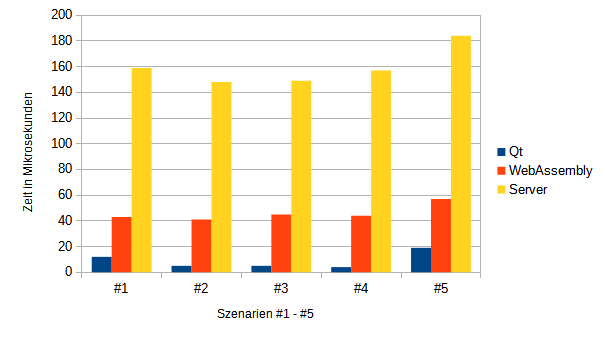
\includegraphics[width=0.9\textwidth, center]{Analyse/Szenarien1_5}
    \caption[Ergebnisse der Szenarien \#1 - \#5 in Microsekunden]{Ergebnisse der Szenarien \#1 -
    \#5
    in Microsekunden}
    \label{img:Szenarien1_5}
\end{figure}
\newline
\newline
\begin{figure}[h]
    \centering
    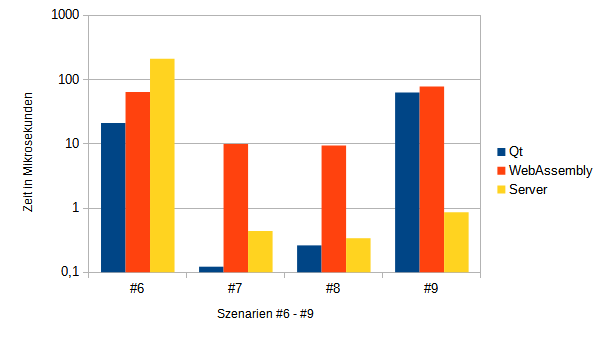
\includegraphics[width=0.9\textwidth, center]{Analyse/Szenarien6_9}
    \caption[Ergebnisse der Szenarien #6 - #9 in Microsekunden]{Ergebnisse der Szenarien #6 - #9
    in Microsekunden}
    \label{img:Szenarien6_9}
\end{figure}
\newpage
\subsection{Tabelle}
\label{subsec:table}
Die Tabelle ist einer der meist genutzten Datenstrukturen um Daten zu repräsentieren. Aus diesem
Grund wurde die Tabelle in der Analyse mit aufgenommen. Dabei wurde eine Tabelle von
\emph{N} Elementen generiert und die Ergebnisse der Messungen im folgenden Diagram zusammengetragen:

\begin{figure}[h]
    \centering
    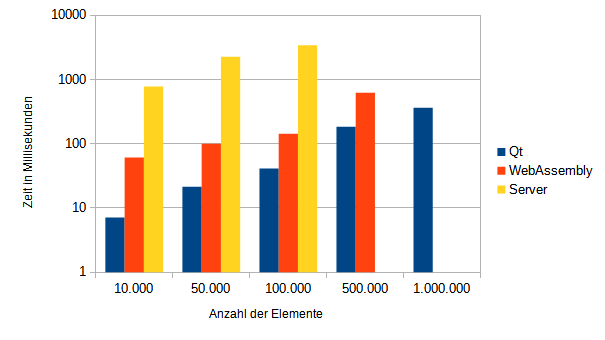
\includegraphics[width=\textwidth, center]{Analyse/Tabelle}
    \caption[Ergebnisse der Messungen von der Erzeugung einer Tabelle in Millisekunden]{Ergebnisse
    der Messungen von der Erzeugung einer Tabelle in Millisekunden}
    \label{img:table}
\end{figure}

Interessant ist zu erkennen, dass die Server-Architektur bei 500.000 Elementen in einem
\emph{Timeout} resultierte. Dieses Vehalten lässt sich dadurch erklären, da die Elemete vom
Server zum Client übertragen werden müssen.

Die WebAssembly-Architektur wiederum, resultierte erst bei 1.000.000 Elementen in einem
\emph{Timeout}. Hier mussten die Elemente nicht zuerst vom Server zum Client übertragen werden,
sondern standen direkt zum Verarbeiten auf dem Client zur Verfügung. Der \emph{Timeout} bei 1.000
.000 Elementen, lässt sich dadurch erklären, dass der \emph{Rendering-Prozess} bei vielen
Elementen zu lange dauert.
\subsection{Baumstruktur}
\label{subsec:tree}
Die Baumstruktur ist dafür gedacht, Elemente zu repräsentieren, die wiederum Unterelemente
enthalten können. Ein klassisches Beispiel ist dabei ein \emph{Filesystem}. Es existieren in
einem \emph{Filesystem} sowohl \emph{Ordner} als auch \emph{Dateien}. Ein \emph{Odner} kann
sowohl mehrere \emph{Dateien} als auch weitere \emph{Ordner} in sich tragen. In den weiteren
\emph{Ordnern} können sich wiederum Elemente befinden.

In diesem Szenario wurden jeweils \emph{NxM} Bäume erzeugt. Dabei steht \emph{N} für die Anzahl
der übergeordneten Elementen und \emph{M} für die Anzahl der untergeordneten Elementen. Die
Ergebnisse der Messungen resultierten in das folgende Diagram:

\begin{figure}[h]
    \centering
    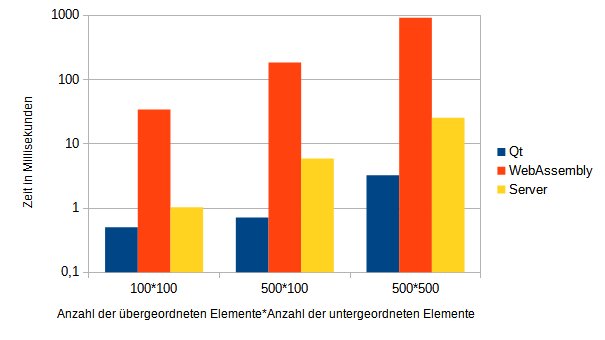
\includegraphics[width=\textwidth, center]{Analyse/Tree}
    \caption[Ergebnisse der Messungen von der Erzeugung einer Baumstruktur in
    Millisekunden]{Ergebnisse
    der Messungen von der Erzeugung einer Baumstruktur in Millisekunden}
    \label{img:table}
\end{figure}

In diesem Diagram ist zu erkennen, das die Server-Architektur performanter als die
WebAssembly-Architektur ist. Dies könnte dadurch erklärt werden, da mit wesentlich weniger
Elementen gearbeitet wurde als in der Sektion \emph{\nameref{subsec:table}}. Dadurch müssen nicht
so viele Elemente vom Server zum Client übertragen werden.
\subsection{Zusammenfassung}
\label{subsec:zusammenfassung}
Das primäre Ziel dieser Laufzeitanalyse war es, die Performance von den zwei \ac{gui}-Frameworks
zu testen. Die Ergebnisse dieser Laufzeitanalyse zeigten, dass Qt Blazor in fast allen
vorgestellten Szenarien überlegen war. Lediglich beim Szenario #9 \emph{Den Text einer Textbox
verändern} zeigte sich, dass die Blazor Server-Architektur leicht überlegen war.
\newline
\newline
Ein möglicher Grund für die Überlegenheit von Qt könnte sein, dass Qt, anders als Blazor, eine
native Desktopanwendung ist. Weitergehend könnte der Faktor, dass C++
eine sehr Hardwarenahe Programmiersprache ist, einen großen Teil zu der Überlegenheit von Qt
beitragen.
\newline
\newline
Interessant war jedoch auch das Verhalten der beiden Blazor-Architekturen zu beobachten. Werden
die ersten sechs vorgestellten Szenarien betrachtet, in denen etwas generiert wurde, dann zeigt
sich, dass die WebAssembly-Architektur wesentlich schneller als die Server-Architektur scheint.
Dies könnte möglicherweise daran liegen, dass die Server-Architektur, die generierten Elemente
erst zum Browser senden muss, damit der Browser diese anzeigen kann.
\newline
\newline
Anders scheint es bei den Szenarien sieben bis neun, bei denen etwas gelesen oder geschrieben
wurde. Dort zeigt sich die Server-Architektur als wesentlich performanter. Hier könnte die
Überlegenheit daran liegen, da die Server-Architektur, die Daten schon lokal zur Verfügung hat
und die Daten direkt verarbeiten kann.
\newline
\newline
Werden die Ergebnisse der Tabellenstruktur und der Baumstruktur gegenübergestellt, so könnte
behauptet werden, dass die Server-Architektur performanter scheint, wenn mit kleineren
Datenmengen gearbeitet wird und die WebAssembly-Architektur dann performanter ist, wenn mit sehr
großen Datenmengen gearbeitet wird.